% !TeX spellcheck = da_DK
\subsection{Forstærker i opsamlingsblok}\label{Subsec:Forstaerker}
\subsubsection{Teori og design}
Til forstærkningen i opsamlingsblokken på \figref{kravblok} skal der benyttes en ikke-inverterende forstærker, da der ønskes, at inputtet og outputtet har samme polaritet. Ved en ikke-inverterende forstærker bliver inputtet tilkoblet direkte til den ikke-inverterende inputterminal, hvilket vil give en høj inputimpedansen, da der kigges direkte ind i operationsforstærkeren. Hvis der var en lav indgangsimpedans, ville denne blok trække meget strøm fra kredsløbet og derved aflade batteriet, der er tiltænkt som spændingsforsyning. \\
Kredsløbet består af en operationsforstærker kaldet LT1028A, som ligner den operationsforstærker, der er tiltænkt at benytte i implementerings delen. Den sidder i et closed-loop med modstandene R$1$ og R$2$, som udgør en spændingsdeler. Dette ses på \figref{fig:Forstaerker}.
\begin{figure}[H]
\centering
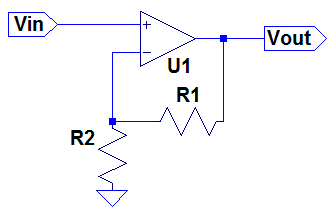
\includegraphics[scale=0.85]{figures/cProblemloesning/Forstaerker.PNG}
\caption{Kredsløbet for en ikke-inverterende forstærker i en closed-loop konfiguration.}
\label{fig:Forstaerker}
\end{figure} 

\noindent Der er jævnført i afsnit \ref{OpsamlingsAfs} på side \pageref{OpsamlingsAfs} bestemt, at forstærkningen skal være en faktor $18$, hvilket svarer til $25.1055$dB. For at udregne R$1$ er R$2$ modstanderen blevet valgt til $10$K$\Omega$. Ud fra dette er R$1$ blevet bestemt ved følgende udregning:
\begin{align}
18 = 1 + (\frac{R1}{10\text{K}\Omega})\\
R1 = 170\text{K}\Omega
\end{align}

\noindent R$1$ og R$2$ bliver brugt til at designe kredsløbet for en ikke-inverterende operations forstærker. Dette kredsløb designes i LT-spice, som ses på \figref{fig:Forstaerker_faktor18}. 
\begin{figure}[H]
\centering
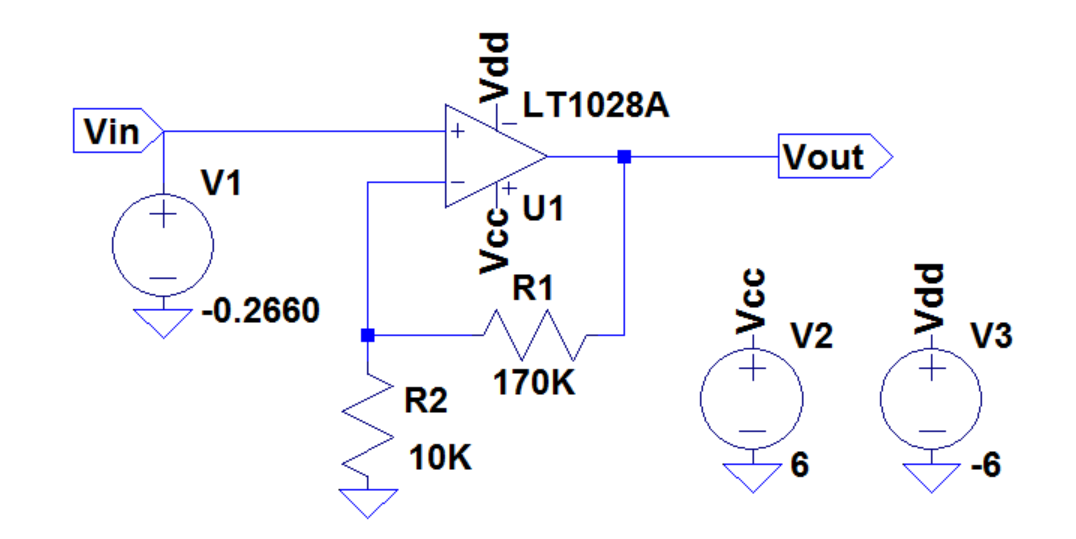
\includegraphics[scale=0.5]{figures/cProblemloesning/Forstaerker_faktor18.PNG}
\caption{Kredsløbet for en ikke-inverterende forstærker med to modstande, R$1$ og R$2$, som med værdierne $10$K$\Omega$ og $170$K$\Omega$ giver en forstærkning med en faktor $18$.}
\label{fig:Forstaerker_faktor18}
\end{figure} 

\subsubsection{Simulering}\label{Subsec:Forstaerker_simu}
Der undersøges i tre simuleringer, om forstærkeren virker ved det laveste input på -$0.2660$V, uden påvirkning ved $0$V samt højeste input på $0.2712$V, som er blevet udregnet igennem pilotforsøget. På \figref{fig:Forstaerker_faktor18_simulering} ses en af de tre simuleringer af spændingerne.

\begin{figure}[H]
\centering
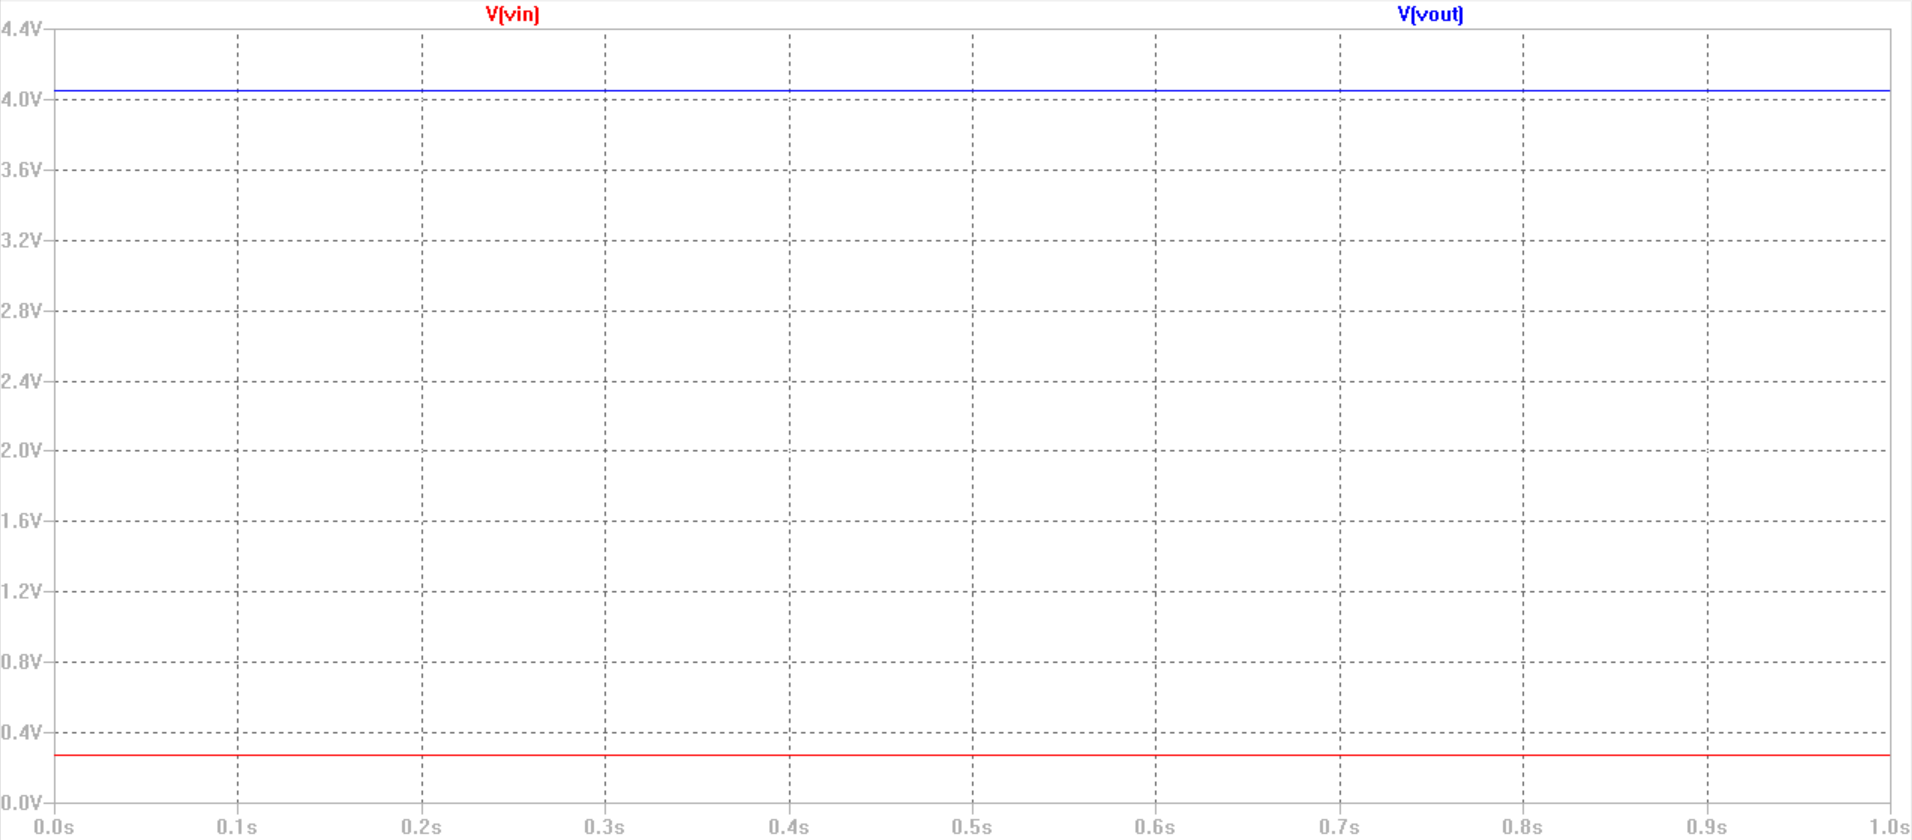
\includegraphics[scale=0.4]{figures/cProblemloesning/Forstaerker_faktor18_simulering.PNG}
\caption{På figuren ses en simuleringen af en ikke-inverterende forstærker, hvor der sker en forstærkning med en faktor $18$. Inputtet, $V_{in}$, er $0.2712$V, som bliver forstærket $18$ gange og derved giver ca. $4.8817$V i outputtet, $V_{out}$.}
\label{fig:Forstaerker_faktor18_simulering}
\end{figure}

Der kan ses på \figref{fig:Forstaerker_faktor18_simulering}, at det forstærkede signal, kaldet $V_{out}$, er ca. $4.8816$V, hvilket er $18$ gange større end $V_{in}$, som i simuleringen er sat til $0.2712$V. Derved er der sket den ønskede forstærkning, hvilket var forventet, da simuleringen er med ideelle komponenter. Derfor har de enkelte komponenter i denne simulering næsten ingen tolerance, hvilket reelle komponenter i et reelt kredsløb vil have mere af. \\
Resultaterne af de tre simuleringer ses i \tableref{tab:forstarker18_sim}
\begin{table}[H]
	\centering
	\begin{tabular}{|l|l|l|l|l|}
		\hline
		\multicolumn{1}{|c|}{\textit{Inputsignalet}} & \multicolumn{1}{c|}{\textit{Forstærkning}} & \multicolumn{1}{c|}{\textit{Forventet outputsignal}} & \multicolumn{1}{c|}{Outputsignalet} & \multicolumn{1}{c|}{\textit{Afvigelse}} \\ \hline
		$0.2712$V      & 18       & $4.8816$V     & $4.8813$V    & $0.0061\%$  \\ \hline
		$0$V           & 18       & $0$V          & $0.000206$V         & $0.0206$\%       \\ \hline
		-$0.2660$V     & 18       & -$4.7880$V    & -$4.7873$V   & $0.0146\%$  \\ \hline
	\end{tabular}
	\caption{Her ses resultaterne for simuleringerne med det laveste-, intet- samt højeste input.}
	\label{tab:forstarker18_sim}
\end{table}
\noindent Der ses på afvigelserne, at der arbejdes med ideelle komponenter, da der er en meget lav afvigelse i outputtet ift. det forventede output. Det er herved bevist, at kredsløbet fungerer teoretisk og kan derfor implementeres.

\subsubsection{Implementering og test}
Der ses på \figref{fig:Forstaerker_faktor18}, at der skal benyttes to modstandere på $10$K$\Omega$ og $170$K$\Omega$ til opbygningen af forstærkeren. Reelt findes der dog ikke en $170$K$\Omega$, hvorfor der istedet benyttes en $270$K$\Omega$ og $470$K$\Omega$ modstander i parallel forbindelse, hvilket teoretisk vil give en $0.874$\% afvigelse fra en ideelt $170$K$\Omega$ modstander. Disse tre modstandere blev målt inden testen, hvilket fremgår i \tableref{Tab:modstand_faktor18}.
\begin{table}[H]
	\centering
	\begin{tabular}{|l|l|l|}
		\hline
		\textit{Teoretisk} & \textit{Ved måling} & \textit{\% afvigelse} \\ \hline
		$10$K$\Omega$       & $10$K$\Omega$        & $0$\%               \\ \hline
		$270$K$\Omega$      & $270.2$K$\Omega$     & $0.01$\%               \\ \hline
		$470$K$\Omega$      & $470$K$\Omega$       & $0$\%               \\ \hline
	\end{tabular}
	\caption{I tabellen ses der, at de tre modstandere afviger lidt fra deres teoretiske værdi, hvilket er forventet af reelle komponenter. Det er dog en acceptabel afvigelse, så modstanderne kan derfor anvendes til implementeringen.}
	\label{Tab:modstand_faktor18}
\end{table}

\noindent Herefter implementeres kredsløbet. Til opsamling af signalet benyttes en computer med ScopeLogger, hvorefter dataen bliver behandlet i Matlab. I testen blev der foretaget 3 målinger for hver af de tre spændingsniveauer. Herefter blev gennemsnittet for hver måling udregnet, som lægges sammen og til slut også tages gennemsnittet af. Dette giver den endelige værdi, som står under "Output" i \tableref{Tab:faktor18_test}.\

\begin{table}[H]
	\centering
	\begin{tabular}{|l|l|l|l|l|}
		\hline
		\textit{Teoretisk input} & \textit{Målte input} & \textit{Forventet output} & \textit{Output} & \% afvigelse \\ \hline
		$0.2712$V   & $0.2715$V    & $4.8870$V     & $4.9292$V       & $0.86\%$     \\ \hline
		$0$V        & $0.289$mV    & $5.202$mV          & $3.2$mV         & $38.49\%$      \\ \hline
		-$0.2660$V  & -$0.2661$V   & -$4.7898$V    & -$4.8341$V      & $0.92\%$     \\ \hline
	\end{tabular}
	\caption{I tabellen ses resultaterne fra testen med forstærkeren, der har en faktor 18}
	\label{Tab:faktor18_test}
\end{table}
Det "målte input" er her blevet målt med et multimeter, da det er nemmere at håndtere end et oscilloskop. For $0.2712$V samt $0$V er spændingen kommet direkte fra en strømforsyning, men for at undersøge forstærkningen af $-0.2660$V er det nødsaget at benytte offsettet, da spændingsforsyningen ikke kan levere en negativ spænding. Det var derfor forventet, at der kunne være en større afvigelse på målingerne med $-0.2660$V spænding, da denne spænding skulle igennem flere kredsløb. Inputtet i offsettet (som kan ses på \figref{fig:Offset_generisk}) var $1.3236$V og referencen var $1.5958$V. Derved skabes den negative spænding, som sendes videre til forstærkeren. Afvigelsen, som ville opstå grundet et ekstra kredsløb, ville være præsentabel for afvigelsen, som der også burde have været for de to andre signalers tests. Der ses i \tableref{Tab:faktor18_test}, at der ikke opstod større forstyrrelser, som gav ekstra afvigelse i det målte signal ift. det forventede signal. \\
Der ses ud fra testen, at forstærkeren overholder kravene fra afsnit \ref{OpsamlingsAfs} på side \pageref{OpsamlingsAfs} samt ligger inde for tolerancerne.